\documentclass{article}
\usepackage[utf8]{inputenc}
\usepackage{graphicx}
\usepackage{here}
\usepackage{amsmath}

\title{Notes de cours\\OPT5 : Apprentissage par renforcement}
\author{Adrien Pavao}
\date{September 2017}

\begin{document}

\maketitle

\section{Introduction}

L'apprentissage par renforcement consiste à apprendre à partir d'expériences, plutôt qu'à partir de données pré-établies, de façon à optimiser une récompense quantitative au cours du temps.

Un agent est plongé au sein d'un environnement. Il doit choisir ses actions (prise de décision) en fonction de son état courant. En retour, l'agent reçoit une récompense de l'environnement, qui peut être positive ou négative.

L'agent cherche à améliorer sa politique de décision au fur et à mesure de sorte à maximiser sa récompense.

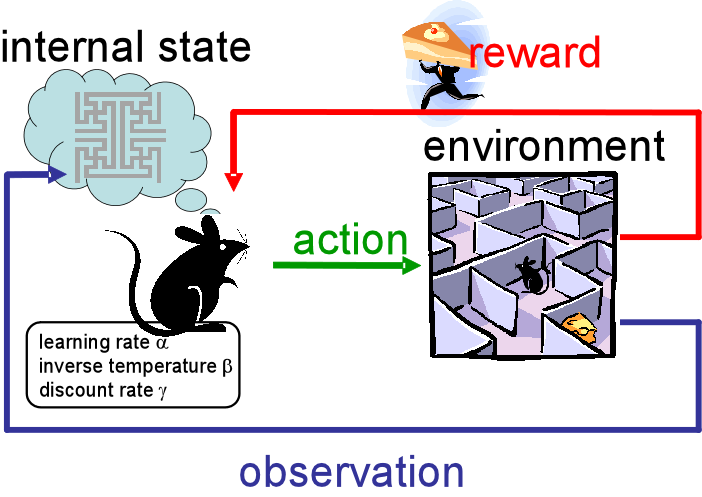
\includegraphics[scale=0.4]{opt5.png}

Dans l'illustration ci-dessus, on voit :
\begin{itemize}
\item \textbf{L'environnement :} Le labyrinthe.
\item \textbf{L'agent :} La souris. C'est l'observation qu'elle fait de l'environnement que l'on nomme son état courant. On nomme tous les états possibles l'\textbf{espace des états}.
\item \textbf{Les actions :} Les actions possibles de la souris en réaction à l'état. Avancer, tourner à gauche, revenir en arrière, etc. Toutes les actions réalisables par l'agent constituent l'\textbf{espace des actions}.
\item \textbf{La récompense :} Le fromage. La souris souhaite tirer profit de sa perception et de sa stratégie de décision afin d'accéder à cette récompense, si possible en un temps minimal.
\end{itemize}

\section{Processus de décision markovien}

Un processus de décision markovien (MDP) est un modèle stochastique où un agent prend des décisions et où les résultats de ses actions sont aléatoires.\footnote{https://fr.wikipedia.org/wiki/Processus\_de\_décision\_markovien}

Formellement, un MDP est un quadruplet ${S, A, T, R}$ :
\begin{itemize}
\item Espace des états S (dénombrable ou continu)
\item Espace des actions A (dénombrable ou continu)
\item Fonction de transition $p(s, a, s') \rightarrow [0, 1]$ (déterministe ou probabiliste)
\item Récompense r(s)
\end{itemize}

On cherche une stratégie $\pi$ qui maximise l'espérance des récompenses cumulées.\\
L'horizon temporelle est notée H et peut être fini (problème épisodique) ou infini (problème coninu).

\section{Equation de Bellman}

A venir.

\end{document}


